\documentclass[10pt,twocolumn,letterpaper]{article}

\usepackage{cvpr}
\usepackage{times}
\usepackage{epsfig}
\usepackage{graphicx}
\usepackage{amsmath}
\usepackage{amssymb}

\usepackage{url}

% Include other packages here, before hyperref.
\usepackage{algorithm}
\usepackage[noend]{algpseudocode}
\usepackage[T1]{fontenc}
\usepackage{fancyref}
\usepackage{float}
% If you comment hyperref and then uncomment it, you should delete
% egpaper.aux before re-running latex.  (Or just hit 'q' on the first latex
% run, let it finish, and you should be clear).
%\usepackage[pagebackref=true,breaklinks=true,letterpaper=true,colorlinks,bookmarks=false]{hyperref}

\cvprfinalcopy % *** Uncomment this line for the final submission

\def\cvprPaperID{****} % *** Enter the CVPR Paper ID here
\def\httilde{\mbox{\tt\raisebox{-.5ex}{\symbol{126}}}}

% Pages are numbered in submission mode, and unnumbered in camera-ready
\ifcvprfinal\pagestyle{empty}\fi
\begin{document}

%%%%%%%%% TITLE
\title{Mean Shift Clustering Algorithm}

\author{Lorenzo Agnolucci\\
E-mail address\\
{\tt\small lorenzo.agnolucci@stud.unifi.it}
% For a paper whose authors are all at the same institution,
% omit the following lines up until the closing ``}''.
% Additional authors and addresses can be added with ``\and'',
% just like the second author.
% To save space, use either the email address or home page, not both
}
\maketitle
\thispagestyle{empty}

%%%%%%%%% ABSTRACT
\begin{abstract}
Mean Shift is a non-parametric clustering technique with a $O(n^{2})$ 		 computational cost, but its embarassingly parallel structure makes it suitable for parallel computing. In this work an OpenMP and a CUDA implementation will be presented and the execution times of each version will be compared. A particular focus will be given to the speedup obtained with the parallel versions for datasets of increasing dimension.
\end{abstract}

%%%%%%%%% BODY TEXT
\noindent\large\textbf{Future Distribution Permission}\\
\indent The author(s) of this report give permission for this document to be distributed to Unifi-affiliated students taking future courses.

\section{Introduction}

\begin{figure*}[!t]
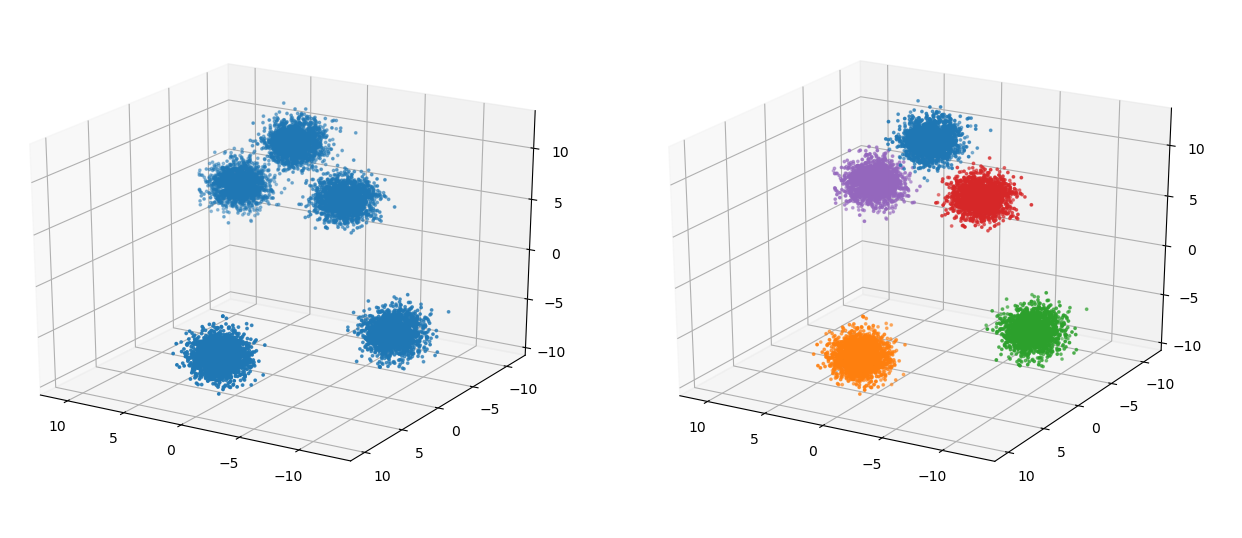
\includegraphics[width=0.99\linewidth]{img/example_combined}
\caption{Example of a dataset with 10000 points respectively not clustered and clustered}
\label{fig:exampleApplication}
\end{figure*}

Mean Shift is a non-parametric clustering algorithm originally presented by Fukunaga and Hostetler \cite{fukunaga1975estimation}. It is based on the \textit{Kernel Density Estimation}, a technique to estimate the underlying probability density function (PDF) of a probability distribution that generated a certain dataset.

The only parameter of the Mean Shift is the \emph{bandwidth}, that controls the smoothing of the resulting PDF (\eg a higher bandwidth will result in fewer but larger clusters). So the main advantage of the Mean Shift is that, unlike K-Means, it does not need to specify the number of clusters. 

At each step a \textit{kernel function} is applied to each point belonging to the dataset to shift it in the direction of the local maxima specified by the kernel. The algorithm ends when all points have reached the maxima of the underlying distribution estimated by the chosen kernel. The set of points shifted to a certain local maximum is identified as a cluster. There are many different types of kernel functions, but the most used is the \textit{Gaussian kernel}:

\begin{align}
K(x) =  e^{-\dfrac{x^2}{2\sigma^2}}
\end{align}

The standard deviation $\sigma$ is the \textit{bandwidth} parameter.

The position in which each point is shifted at each step of the algorithm is computed as a weighted average between the point and all the others, where the weights are calculated with a given kernel function. Suppose $x$ is a point to be shifted and  $N(x)$ is the neighborhood of $x$, a set of points for which K($x_i$) $\neq$ 0. Let $dist(x, x_i)$ be the distance from the point $x$ to the point $x_i$. The new position $x'$ where $x$ has to be shifted is computed as follows \cite{Wiki}:

\begin{align}
x' = \dfrac{\sum_{x_i \in N(x)} K(dist(x,x_i)) x_i}{\sum_{x_i \in N(x)} K(dist(x, x_i))}
\end{align}



The mean shift algorithm applies that formula to each point iteratively until they converge, that is until the position does not change. This means that all the points have reached their corresponding local maximum of the underlying distribution. The algorithm ends when all the points have stopped shifting.

The idea behind the algorithm shows that Mean Shift is embarassingly parallel, because each point can be processed distinctly from the others. This suggests that it is convenient to build a parallel version: this work presents two different parallel implementations, one with OpenMP and the other with CUDA.
Also, Mean Shift has a computational cost of $O(n^{2})$, so making it parallel can compensate for the increasing execution time and make it suitable for problems with a lot of data.

%-------------------------------------------------------------------------%-------------------------------------------------------------------------

\section{Proposed approach}
The proposed sequential implementation is a simple translation of the principle behind the Mean Shift in C++. The \textbf{Gaussian kernel} has been chosen as the kernel function and the Euclidean distance has been used to measure the distance between two points. Since the Guassian kernel can't be equal to zero the neighbors of each point are all the other points. The \emph{Algorithm \ref{MeanShiftAlgSeq}} shows the pseudocode of the core of the algorithm:

\begin{algorithm}
\caption{Mean shift core}
\label{MeanShiftAlgSeq}
\begin{algorithmic}
\Function{MeanShift}{$originalPoints$}
	\State$shiftedPoints \gets originalPoints$
    \While{iterationIndex $<$ $MAX\_ITERATIONS$}
            \For{each point $p$ in $shiftedPoints$}
               \State $p\gets \Call{ShiftPoint}{p, originalPoints}$
            \EndFor
    \EndWhile
\EndFunction
\end{algorithmic}
\end{algorithm}

\begin{algorithm}
\caption{Shift a single point}
\label{ShiftPointAlgSeq}
\begin{algorithmic}
\Function{ShiftPoint}{$p, originalPoints$}
	\State $shiftedP\gets0$
	\State $weight\gets0$
    \For{each point $x$ in $originalPoints$}
    		\State$dist \gets dist(p, x)$
    		\State $w \gets GKernel(dist, BW)$
    		\State $shiftedP \gets shiftedP + w*x$
    		\State $weight \gets weight + w$
    \EndFor
    \State \textbf{return} $shiftedP/weight$
\EndFunction

\end{algorithmic}
\end{algorithm}

The $MAX\_ITERATIONS$ constant represents the number of times each point is shifted, while the BW constant stands for the bandwidth. In this implementation the algorithm is built to work specifically with 3D points (even if modifying it to make it work with other dimensions would be trivial) because a common application of Mean Shift in \emph{Computer Vision} is \emph{Image Segmentation} on RGB images \cite{comaniciu1999mean}.

\emph{Figure \ref{fig:exampleApplication}} shows a dataset with 10000 points respectively not clustered and clustered with the algorithm.

%-------------------------------------------------------------------------

\subsection{OpenMP version}
Using the OpenMP library lets to transform the sequential version into a parallel one with a single \textbf{pragma} directive. Indeed, as can be seen in \emph{Algorithm \ref{OpenMPAlgorithm}}, the OpenMP implementation differs from the sequential one for just a statement.

\begin{algorithm}
\caption{OpenMP Mean shift core}
\label{OpenMPAlgorithm}
\begin{algorithmic}
\Function{OpenMPMeanShift}{$originalPoints$}
	\State$shiftedPoints \gets originalPoints$
    \While{iterationIndex $<$ $MAX\_ITERATIONS$}
    			\State \#pragma parallel for schedule(static)
            \For{each point $p$ in $shiftedPoints$}
               \State $p\gets \Call{ShiftPoint}{p, originalPoints}$
            \EndFor
    \EndWhile
\EndFunction
\end{algorithmic}
\end{algorithm}

The pragma directive is used just before the \emph{for} loop: in this way there is no need of any critical section because in each iteration each point is shifted indipendently from the others. It is important to note that a \textbf{static scheduling} has been used because in this way the \emph{for} loop is divided statically in chunks of equal size, and this assures that each thread receives the same workload because the number of iterations is fixed from the start.

%-------------------------------------------------------------------------

\subsection{CUDA version}
Implementing the algorithm with CUDA lets to take advantage of the great number of cores of GPUs. Indeed the processing of each point can be assigned to a different thread. In this work two different versions will be presented: a naive one and a more optimized one that uses tiling and shared memory. From now on it will be used the CUDA terminology \cite{CUDADocs}.

The array of the points has only one dimension, so both the blocks and the grid require only the \emph{x} coordinate to be defined. In particular, \emph{blockDim.x} will be equal to a constant $BLOCK\_DIM$, while the number of blocks will be $\lceil numPoints / BLOCK\_DIM \rceil$.

Both the proposed implementations are built to exploit the fact that modern DRAM systems are designed to always be accessed in burst mode. In fact the points are stored in memory as a \emph{Structure of Arrays} to allow \textbf{coalescing} and to be more L2 cache friendly (in contrast to \emph{Arrays of Structures} and the corresponding strided access):

\begin{align}
[x_{}, \ldots , x_{n}, y_{1}, \ldots, y_{n}, z_{1}, \ldots , z_{n}]
\end{align}

Moreover, the access to the array is in the form of:

\begin{align}
blockDim.x*blockIdx.x+threadIdx.x
\end{align}

For these reasons all threads in a warp access to consecutive global memory locations. This lets the hardware to coalesce all the accesses into a consolidated access to consecutive DRAM locations increasing performances.


%-------------------------------------------------------------------------
\subsubsection{Naive version}
\label{naiveSection}
In the naive version the algorithm is simply implemented as a CUDA kernel. A wrapper function is also necessary to call the kernel the number of times specified by $MAX\_ITERATIONS$. The wrapper and the kernel can be seen respectively in \emph{Algorithm \ref{NaiveCUDAMeanShiftAlg}} and \emph{\ref{NaiveCUDAKernelAlg}}.

\begin{algorithm}
\caption{CUDA Naive version Mean Shift core}
\label{NaiveCUDAMeanShiftAlg}
\begin{algorithmic}
\Function{NaiveCUDAMS}{$originalPoints$}
	\State$shiftedPoints \gets originalPoints$
    \While{iterationIndex $<$ $MAX\_ITERATIONS$}
    		\State $\Call{NaiveKernel}{shiftedPoints, originalPoints}$
    \EndWhile
\EndFunction
\end{algorithmic}
\end{algorithm}


\begin{algorithm}
\caption{CUDA Naive version Kernel }
\label{NaiveCUDAKernelAlg}
\begin{algorithmic}
\Function{NaiveKernel}{$shiftedPts, originalPts$}
	\State $tx \gets threadIdx.x$
	\State $bx \gets blockIdx.x$
	\State $idx \gets bx * blockDim.x + tx$
	\If{$idx < |originalPts|$}
	\State $shiftedP \gets 0$
	\State $weight \gets 0$
	\State $p \gets shiftedPts[idx]$
    \For{each point $x$ in $originalPts$}
    		\State$dist \gets dist(p, x)$
    		\State $w \gets GKernel(dist, BW)$
    		\State $shiftedP\gets shiftedP + w*x$
    		\State $weight \gets weight + w$
    \EndFor
    \State $shiftedPts[idx] \gets shiftedP/weight$
    \EndIf
\EndFunction
\end{algorithmic}
\end{algorithm}

Before computing the shift of its corresponding point each thread has to check if its index is not greater that the number of points: in this case the thread simply does nothing. This happens when the number of points is not multiple of $BLOCK\_DIM$, therefore more threads have been instantiated than necessary.

%-------------------------------------------------------------------------

\subsubsection{Tiling version}
Starting from the naive version a more optimized implementation can be developed. Indeed in the \emph{Algorithm \ref{NaiveCUDAKernelAlg}} can be seen that each thread to compute the shift needs to access \emph{O(n)} times in global memory, one for each point. This results in a loss of performance caused by the relatively slow access to global memory.
 
A way to overcome this problem is to exploit the \textbf{Shared Memory} with the \emph{Tiling} pattern, relying on the fact that the original points are read by all the threads but not modified. At first, during the loading phase, each thread loads into the Shared Memory the point which was assigned to, and then it computes a partial shift based on only the points contained in the current tile. Due to the limited amout of Shared Memory (48KB per block, 96KB per \emph{Streaming Multiprocessors} for the \emph{Pascal Architecture} \cite{Pascal}) this process must be repeated for several iterations, until all the points are loaded and used to compute the shift. Let $TILE\_WIDTH = BLOCK\_DIM$ be the number of points contained at once in the Shared Memory, then each thread reduces the number of accesses to the global memory from $O(n)$ to $O(n/TILE\_WIDTH)$.

As explained previously in section \ref{naiveSection}, both a wrapper function and a kernel exploiting Shared Memory have been developed (respectively \emph{Algorithm \ref{TilingCUDAMeanShiftAlg}} and \emph{Algorithm \ref{TilingCUDAKernelAlg}}).

\begin{algorithm}
\caption{CUDA Tiling version Mean Shift core}
\label{TilingCUDAMeanShiftAlg}
\begin{algorithmic}
\Function{TilingCUDAMS}{$originalPoints$}
	\State$shiftedPoints \gets originalPoints$
    \While{iterationIndex $<$ $MAX\_ITERATIONS$}
    		\State $\Call{TilingKernel}{shiftedPoints, originalPoints}$
    \EndWhile
\EndFunction
\end{algorithmic}
\end{algorithm}


\begin{algorithm}
\caption{CUDA Tiling version Kernel }
\label{TilingCUDAKernelAlg}
\begin{algorithmic}
\Function{TilingKernel}{$shiftedPts, originalPts$}
	\State $tx \gets threadIdx.x$
	\State $bx \gets blockIdx.x$
	\State $idx \gets bx * blockDim.x + tx$
	\State $tile \gets SharedMemArray[TILE\_WIDTH]$
	\State $shiftedP \gets 0$
	\State $weight \gets 0$
	\For{$tileIter < numTiles$}
		\State$tileIdx \gets tileIter * TILE\_WIDTH + tx$
		\If{$idx < |originalPts|$}
			\State$tile[tx] \gets originalPts[tileIdx]$
		\Else
			\State$tile[tx] \gets nullPoint$
		\EndIf
		\State$\_\_synchthreads()$\Comment{End of loading}
		\If{$idx < |originalPts|$}
			\State $p \gets shiftedPts[idx]$
    			\For{$i$ with $i < TILE\_WIDTH$}
    				\State $x \gets tile[i]$
    				\If{$x != nullPoint$}
    					\State $dist \gets dist(p, x)$
    					\State $w \gets GKernel(dist, BW)$
    					\State $shiftedP\gets shiftedP + w*x$
    					\State $weight \gets weight + w$
    				\EndIf
    			\EndFor
    		\EndIf
    		\State$\_\_synchthreads()$\Comment{End of computing}
	\EndFor
	\If{$idx < |originalPts|$}
    		\State $shiftedPts[idx] \gets shiftedP/weight$
    	\EndIf
    
\EndFunction
\end{algorithmic}
\end{algorithm}

\emph{Algorithm \ref{TilingCUDAKernelAlg}} presents some points of particular interest:
\begin{itemize}
\item two indexes are required: \emph{idx} refers to the shifting point which the thread was assigned to, \emph{tileIdx} represents the point that the thread has to load into the Shared Memory
\item the two $\_\_syncthreads()$ represent necessary thread barriers: the first one assures that each thread has loaded the corresponding point to the Shared Memory before the computing, the second one guarantees that all the threads have computed the partial shift before the next iteration
\item during the loading phase a boundary check is performed: if a thread is to load a point that is not in the valid index range it loads a dummy point with a flag value. Then, during the computing of the partial shift, each thread checks if the current point is a dummy one and in that case it simply ignores it: in this way the dummy points will not affect the final value of the shifting point.
\end{itemize}

%-------------------------------------------------------------------------
%-------------------------------------------------------------------------

\section{Experimental results}
The metric used to compare the performances of the sequential algorithm with the OpenMP and the CUDA versions is the \textbf{speedup}, computed as:
\begin{align}
S = \dfrac{t_S}{t_P}
\end{align}
where $t_S$ and $t_P$ are respectively the execution time of the sequential and the parallel implementation.

The datasets used to evaluate the different implementations have been generated with the \emph{$make\_blob$} function of \emph{sklearn.datasets} \cite{scikit-learn}. They are gaussian distributions with 5 centers and standard deviation equal to 1 and are composed by respectively 100, 1000, 10000, 100000 and 250000 3D points.

The $MAX\_ITERATIONS$ constant has been set to 10 because it has been estimated empirically that 10 iterations are enough to make all the points converge to the local maxima, while the value associated to the BW (i.e. bandwidth) constant was 2.

The tests have been executed on a machine with:
\begin{itemize}
\item OS: Ubuntu 18.04 LTS
\item CPU: Intel Core i7-8565U 1.8GHz up to 4.6GHz with Turbo Boost, 4 cores/8 threads
\item RAM: 16 GB DDR4
\item GPU: NVidia GeForce MX250 2GB with CUDA 10.1
\end{itemize}

To make the results more reliable and representative each execution time has been obtained as the average of the times measured running each test 5 times for the sequential and the OpenMP versions and 15 times for each CUDA implementation. 
%-------------------------------------------------------------------------
\subsection{OpenMP}
To evaluate the performances of the OpenMP implementation it has been executed on each dataset with an increasing number of threads. The results for the 100, 1000, 10000 and 10000 dataset are shown respectively in \emph{figure \ref{fig:chart100points}} and \emph{table \ref{tab:table100points}}, \emph{figure \ref{fig:chart1000points}} and \emph{table \ref{tab:table1000points}}, \emph{figure \ref{fig:chart10000points}} and \emph{table \ref{tab:table10000points}}, \emph{figure \ref{fig:chart100000points}} and \emph{table \ref{tab:table100000points}}. Unfortunately both the sequential and the OpenMP implementations could not be executed on the 250000 points dataset because it would have taken too much time, so they have been estimated (as explained later).

\begin{figure}
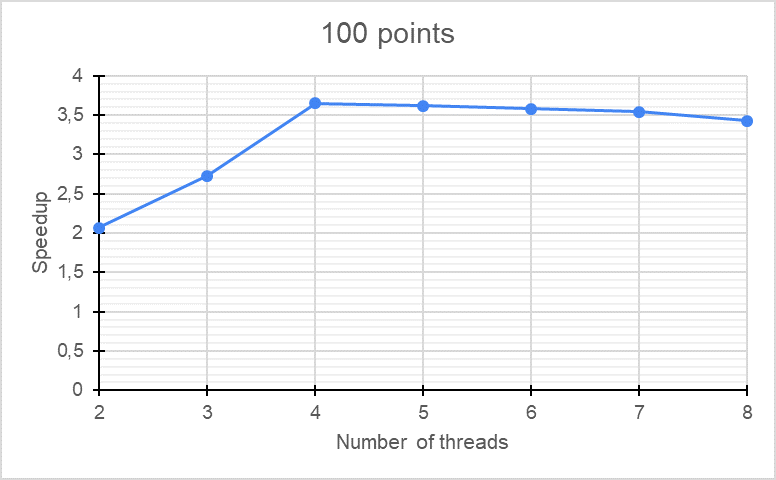
\includegraphics[width=0.99\linewidth]{img/chart_100_points}
\caption{Speedup for 100 points varying the number of threads with OpenMP}
\label{fig:chart100points}
\end{figure}

\begin{table}[]
\centering
\begin{tabular}{|c|c|c|}
\hline
\textbf{Dim} & \multicolumn{2}{c|}{100} \\ \hline
\textbf{Sequential} & \multicolumn{2}{c|}{0.005384 s} \\ \hline
\textbf{Thread} & \textbf{Time} & \textbf{Speedup} \\ \hline
2 & 0.002607 s & 2.07 \\ \hline
3 & 0.001973 s & 2.73 \\ \hline
4 & \textbf{0.001473 s} & \textbf{3.66} \\ \hline
5 & 0.001487 s & 3.62 \\ \hline
6 & 0.001503 s & 3.58 \\ \hline
7 & 0.001519 & 3.55 \\ \hline
8 & 0.001570 & 3.43 \\ \hline
\end{tabular}
\caption{Speedup for 100 points varying the number of threads with OpenMP (best result in bold)}
\label{tab:table100points}
\end{table}

\begin{figure}
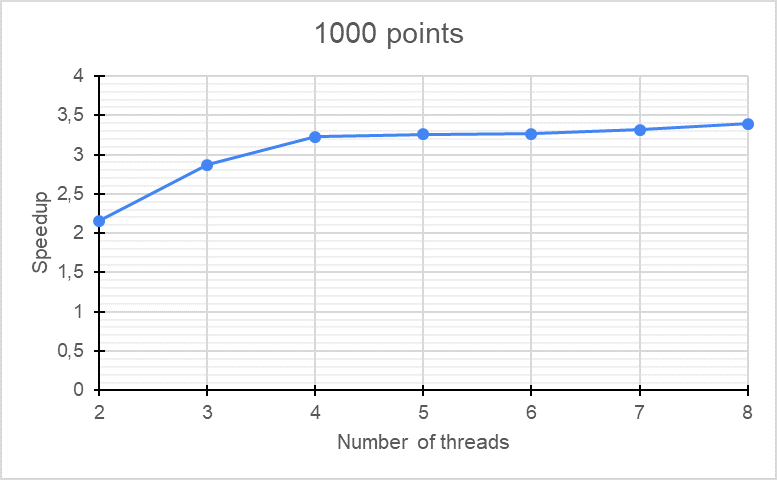
\includegraphics[width=0.99\linewidth]{img/chart_1000_points}
\caption{Speedup for 1000 points varying the number of threads with OpenMP}
\label{fig:chart1000points}
\end{figure}

\begin{table}[]
\centering
\begin{tabular}{|c|c|c|}
\hline
\textbf{Dim} & \multicolumn{2}{c|}{1000} \\ \hline
\textbf{Sequential} & \multicolumn{2}{c|}{0.475485 s} \\ \hline
\textbf{Thread} & \textbf{Time} & \textbf{Speedup} \\ \hline
2 & 0.220345 s & 2.16 \\ \hline
3 & 0.165760 s & 2.87 \\ \hline
4 & 0.147428 s & 3.23 \\ \hline
5 & 0.145838 s & 3.26 \\ \hline
6 & 0.145555 s & 3.27 \\ \hline
7 & 0.143497 s & 3.32 \\ \hline
8 & \textbf{0.140161 s} & \textbf{3.39} \\ \hline
\end{tabular}
\caption{Speedup for 1000 points varying the number of threads with OpenMP (best result in bold)}
\label{tab:table1000points}
\end{table}

\begin{figure}
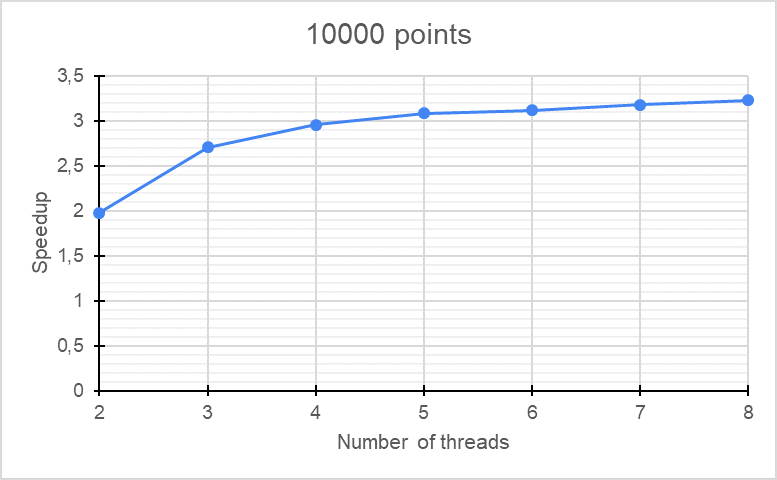
\includegraphics[width=0.99\linewidth]{img/chart_10000_points}
\caption{Speedup for 10000 points varying the number of threads with OpenMP}
\label{fig:chart10000points}
\end{figure}

\begin{table}[]
\centering
\begin{tabular}{|c|c|c|}
\hline
\textbf{Dim} & \multicolumn{2}{c|}{10000} \\ \hline
\textbf{Sequential} & \multicolumn{2}{c|}{49.29 s} \\ \hline
\textbf{Thread} & \textbf{Time} & \textbf{Speedup} \\ \hline
2 & 24.91 s & 1.98 \\ \hline
3 & 18.21 s & 2.71 \\ \hline
4 & 16.64 s & 2.97 \\ \hline
5 & 15.96 s & 3.09 \\ \hline
6 & 15.78 s & 3.13 \\ \hline
7 & 15.48 s & 3.19 \\ \hline
8 & \textbf{15.25 s} & \textbf{3.24} \\ \hline
\end{tabular}
\caption{Speedup for 10000 points varying the number of threads with OpenMP (best result in bold)}
\label{tab:table10000points}
\end{table}

\begin{figure}
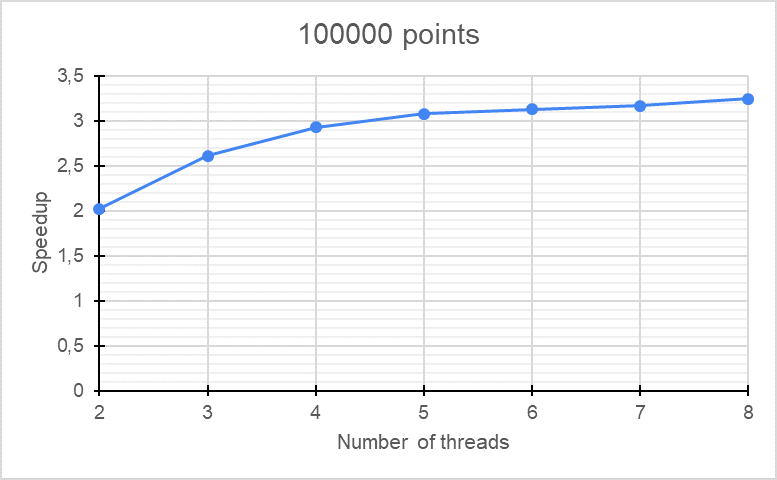
\includegraphics[width=0.99\linewidth]{img/chart_100000_points}
\caption{Speedup for 100000 points varying the number of threads with OpenMP}
\label{fig:chart100000points}
\end{figure}

\begin{table}[]
\centering
\begin{tabular}{|c|c|c|}
\hline
\textbf{Dim} & \multicolumn{2}{c|}{100000} \\ \hline
\textbf{Sequential} & \multicolumn{2}{c|}{4560.37 s} \\ \hline
\textbf{Thread} & \textbf{Time} & \textbf{Speedup} \\ \hline
2 & 2252.48 s & 2.03 \\ \hline
3 & 1744.97 s & 2.62 \\ \hline
4 & 1554.59 s & 2.94 \\ \hline
5 & 1479.61 s & 3.09 \\ \hline
6 & 1456.03 s & 3.14 \\ \hline
7 & 1437.89 s & 3.18 \\ \hline
8 & \textbf{1403.78 s} & \textbf{3.25} \\ \hline
\end{tabular}
\caption{Speedup for 100000 points varying the number of threads with OpenMP (best result in bold)}
\label{tab:table100000points}
\end{table}

For the 100 points dataset (\emph{figure \ref{fig:chart100points}} and \emph{table \ref{tab:table100points}}) interestingly the speedup decreases for more than 4 threads. This shows how for such a low number of points the overhead of the threads outweighs the gain from using them. As expected this phenomenon disappears for the datasets with more points and the use of more threads lowers the execution time (and consequently increases the speedup). 
The results show how OpenMP lets to reach a speedup equal to atleast \textbf{3} at the expense of a single pragma directive, so OpenMP proves to have an excellent speedup and development cost ratio.


%-------------------------------------------------------------------------
\subsection{CUDA}

The first test was aimed at finding the optimal $TILE\_WIDTH$ (and also $BLOCK\_DIM$ because $TILE\_WIDTH = BLOCK\_DIM$), so different execution times were measured for a dataset with 100000 points increasing $TILE\_WIDTH$. As \emph{figure \ref{fig:chartTileWidth}} and \emph{table \ref{tab:tableCudaSpeedup}} show, the best time was obtained for $TILE\_WIDTH = 64$ so it was used for the other tests.

\begin{figure}
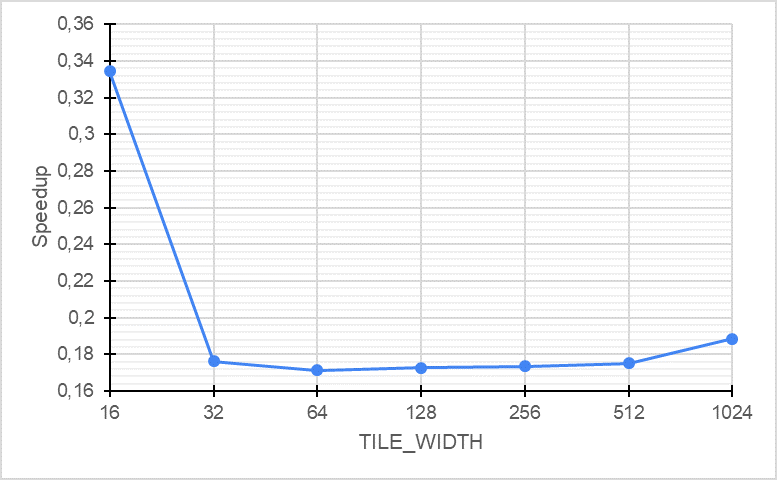
\includegraphics[width=0.99\linewidth]{img/chart_tile_width}
\caption{Execution time for 10000 points for the CUDA tiling implementation varying $TILE\_WIDTH$}
\label{fig:chartTileWidth}
\end{figure}

\begin{table}[]
\centering
\begin{tabular}{|c|c|}
\hline
\textbf{\textbf{TILE$\_$WIDTH}} & \textbf{CUDA Tiling} \\ \hline
16 & 0.334405 s \\ \hline
32 & 0.176171 s \\ \hline
\textbf{64} & \textbf{0.171354 s} \\ \hline
128 & 0.172666 s \\ \hline
256 & 0.173306 s \\ \hline
512 & 0.175091 s \\ \hline
1024 & 0.18845 s \\ \hline
\end{tabular}
\caption{Execution time for 10000 points for the CUDA tiling implementation varying $TILE\_WIDTH$ (best result in bold)}
\label{tab:tableCudaSpeedup}
\end{table}

\begin{table*}[]
\centering
\begin{tabular}{|c|c|c|c|c|c|c|}
\hline
\textbf{Dim} & \multicolumn{2}{c|}{\textbf{Sequential}} & \textbf{OpenMP} & \textbf{OpenMP Speedup} & \textbf{CUDA Tiling} & \textbf{CUDA Speedup} \\ \hline
100 & \multicolumn{2}{c|}{0.005384 s} & 0.001473 s & 3.66 & 0.000401 s & 13.43 \\ \hline
1000 & \multicolumn{2}{c|}{0.475485 s} & 0.140161 s & 3.39 & 0.003044 s & 156.21 \\ \hline
10000 & \multicolumn{2}{c|}{49.29 s} & 15.25 s & 3.24 & 0.171354 s & 287.64 \\ \hline
100000 & \multicolumn{2}{c|}{4560.37 s} & 1403.78 s & 3.25 & 15.79 s & 288.80 \\ \hline
250000 & \multicolumn{2}{c|}{$\dagger$ 27768 s} & $\dagger$ 8720 s & $\dagger$ 3.18 & 100.38 s & $\dagger$ 276.61 \\ \hline
\end{tabular}
\caption{Global comparison between sequential, OpenMP and Tiling CUDA best results varying dataset dimension ($\dagger$ times and speedups are estimated)}
\label{tab:globalComparison}
\end{table*}

\begin{table}[]
\centering
\begin{tabular}{|c|c|c|c|}
\hline
\textbf{Dim} & \textbf{CUDA Naive} & \textbf{CUDA Tiling} & \textbf{Speedup} \\ \hline
100 & 0.000401 s & 0.000437 s & 1.09 \\ \hline
1000 & 0.003044 s & 0.003359 s & 1.11 \\ \hline
10000 & 0.171354 s & 0.191216 s & 1.12 \\ \hline
100000 & 15.79 s & 18.29 s & 1.16 \\ \hline
250000 & 100.38 s & 121.10 s & 1.20 \\ \hline
\end{tabular}
\caption{Execution time and speedup obtained with naive and tiling CUDA implementations for increasing dataset dimension}
\label{tab:naiveTilingSpeedup}
\end{table}

\begin{table}[]
\centering
\begin{tabular}{|c|c|c|c|}
\hline
\textbf{Dim} & \textbf{Sequential} & \textbf{CUDA Tiling} & \textbf{Speedup} \\ \hline
100 & 0.005384 s & 0.000401 s & 13.43 \\ \hline
1000 & 0.475485 s & 0.003044 s & 156.21 \\ \hline
10000 & 49.29 s & 0.171354 s & 287.64 \\ \hline
100000 & 4560.37 s & 15.79 s & 288.80 \\ \hline
250000 & $\dagger$ 27768 s & 100.38 s & $\dagger$ 276.61 \\ \hline
\end{tabular}
\caption{Execution time and speedup obtained with sequential and tiling CUDA implementations for increasing dataset dimension ($\dagger$ times and speedups are estimated)}
\label{tab:cudaSpeedup}
\end{table}

Then both the naive and the tiling version was executed on all the datasets. In \emph{\fref{tab:naiveTilingSpeedup}} can be seen that exploiting the Shared Memory with the tiling pattern lets to increase the performances of a respectable amount.

The final test was focused on the actual speedup of the tiling CUDA implementation in relation to the sequential algorithm. \emph{\Fref{tab:cudaSpeedup}} clearly shows how the use of GPUs lets to considerably increase the performances and to apply the algorithm to otherwise intractable datasets. Indeed it is important to note that the execution time for the 250000 points dataset was not measured but estimated with a quadratic regression (due to the $O(n^{2})$) because repeating the test for 5 times would have taken too much time. As expected for datasets with a low number of points (\ie 100 and 1000) the maximum potential of the GPU is not expressed, but then for bigger datasets the speedup increases and stabilize at about \textbf{288} when the technical characteristics of the GPU become limiting.


\subsection{Comparison}

As a final result a global comparison has been conducted and therefore only the best results for each dataset dimension and each implementation have been considered. It is important to note that since the execution time for the 250000 points dataset of the OpenMP implementation was not measured it has been estimated using a quadratic regression and then the corresponding speedup has been computed. In \emph{\fref{tab:globalComparison}} can be seen that the CUDA algorithm abundantly \textbf{outperforms} both the sequential and the OpenMP ones, at the expense of a more complicated implementation. However OpenMP lets to achieve a noticeable speedup with just a single directive.


%-------------------------------------------------------------------------
%-------------------------------------------------------------------------
\section{Conclusions}
In this work the Mean Shift clustering algorithm was presented and it was shown how its embarassingly parallel structure makes it suitable for parallel computing. A parallel implementation with OpenMP was developed by adding just a directive and it let to obtain a speedup equal to more than 3. Then a CUDA implementation (in a naive version and in a more optimized one that uses tiling) was presented and with its about 288 speedup showed how the use of GPUs makes Mean Shift applicable to datasets intractable with a CPU.
%-------------------------------------------------------------------------

{\small
\bibliographystyle{ieee}
\bibliography{egbib}
}
\end{document}
